\documentclass{article}
\usepackage{graphicx}
\usepackage{amsmath}
\usepackage{subfigure}

\begin{document}

\begin{figure}[ht]
\centering

%
\subfigure
[
A trace.
]
{
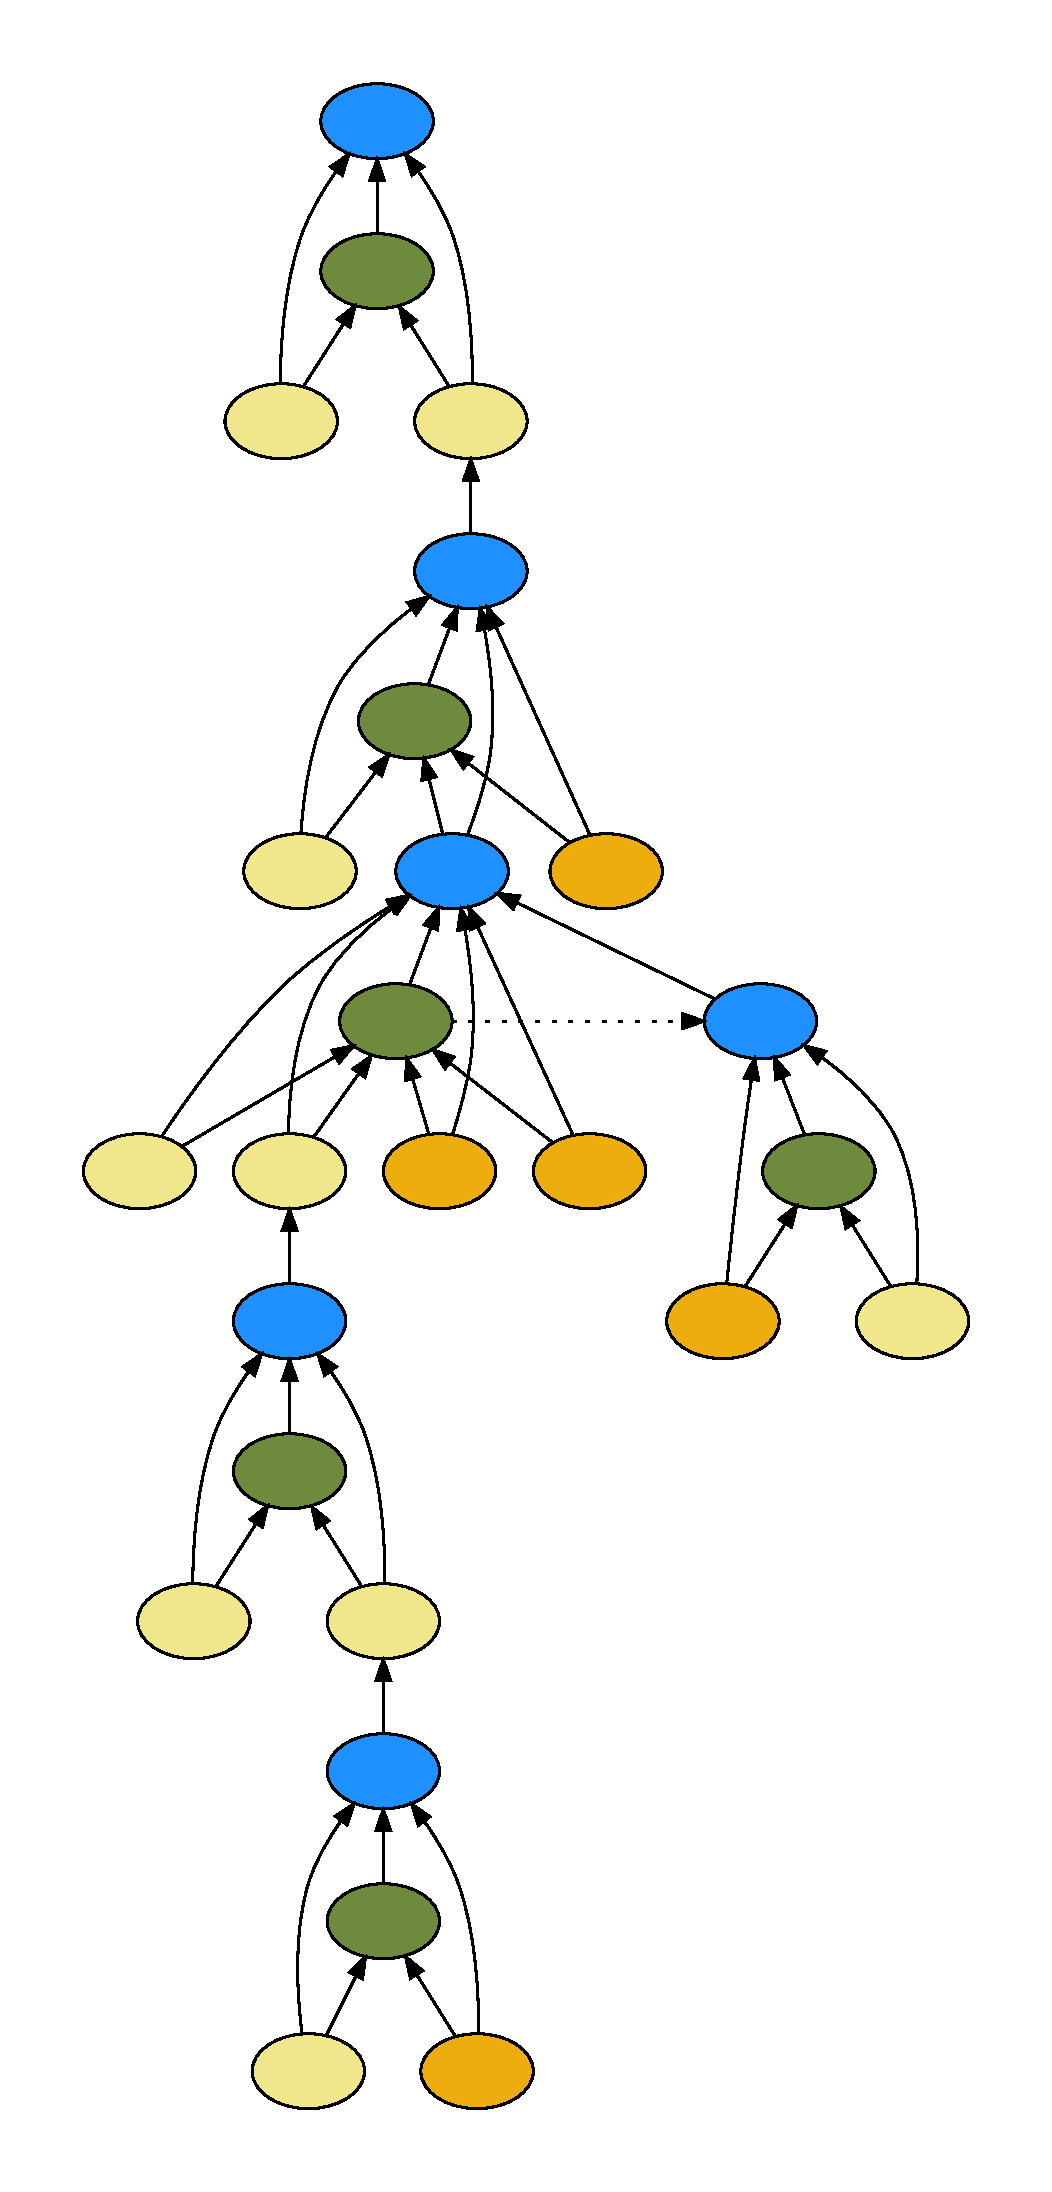
\includegraphics[width=200pt,height=200pt]{partition/dot0.pdf}

\label{fig:partition_rho}
}

\quad

\subfigure
[
The scaffold partitions the trace into five groups: 
]
{
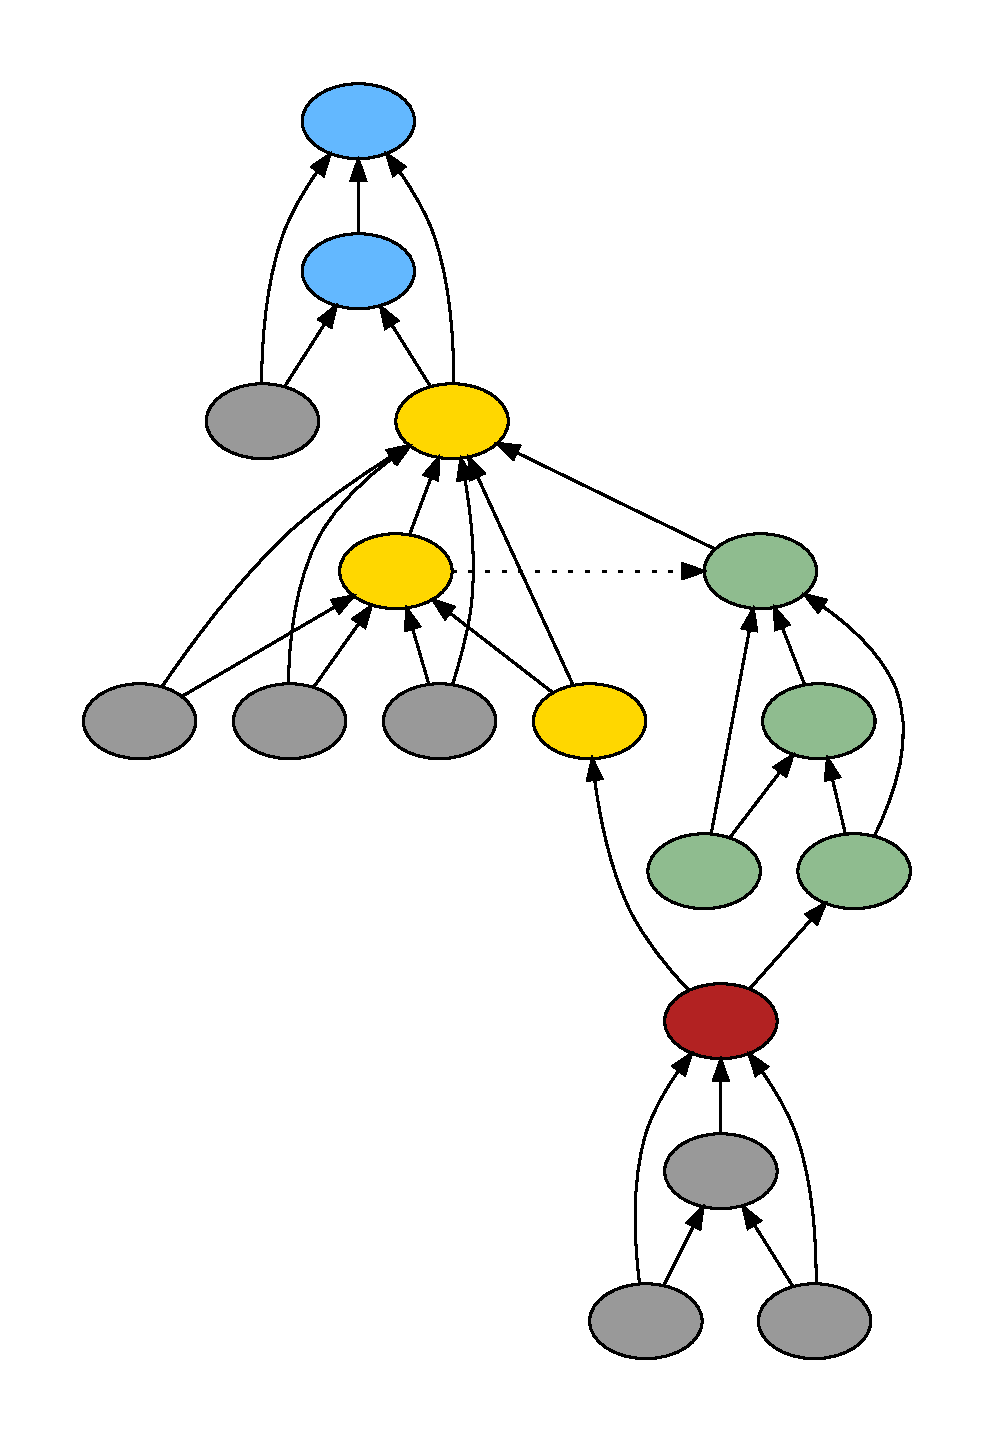
\includegraphics[width=200pt,height=200pt]{erg_to_drg/dot2.pdf}
\label{fig:scaffold_disabled}

}

%

\caption{The two stages of constructing a scaffold}

\label{fig:partition}
\end{figure}



%%%%%%%%%%%%%%%%%%%%%%%%%%%%%%%%
%%%%%%%%%%%%%%%%%%%%%%%%%%%%%%%%
%%%%%%%%%%%%%%%%%%%%%%%%%%%%%%%%
\begin{figure}[ht]
\centering

%
\subfigure
[
First we walk downstream from the principal node, and color gold every node
whose value may change, and blue every node at which we can
absorb.
]
{
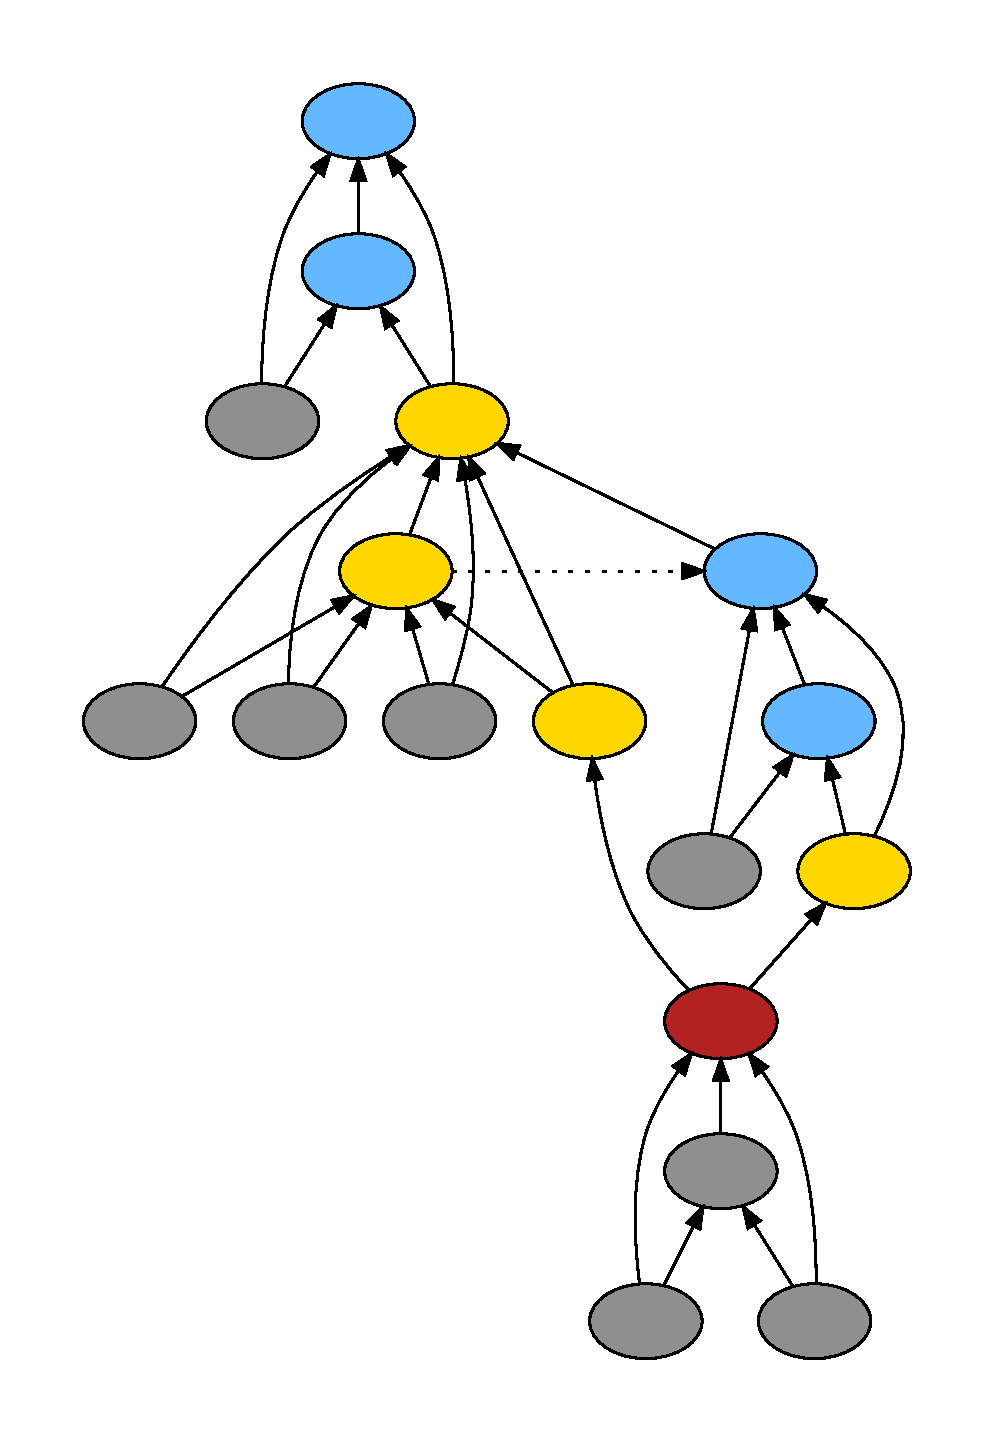
\includegraphics[width=200pt,height=200pt]{erg_to_drg/dot4.pdf}

\label{fig:scaffold_extended}
}

\quad

\subfigure
[
Next, we color green every node that may no longer exist once
the gold nodes are resampled. At this point, the red and gold nodes 
constitute the definite regeneration graph, the blue nodes constitute the absorbing border, and the green nodes constitute the brush.
]
{
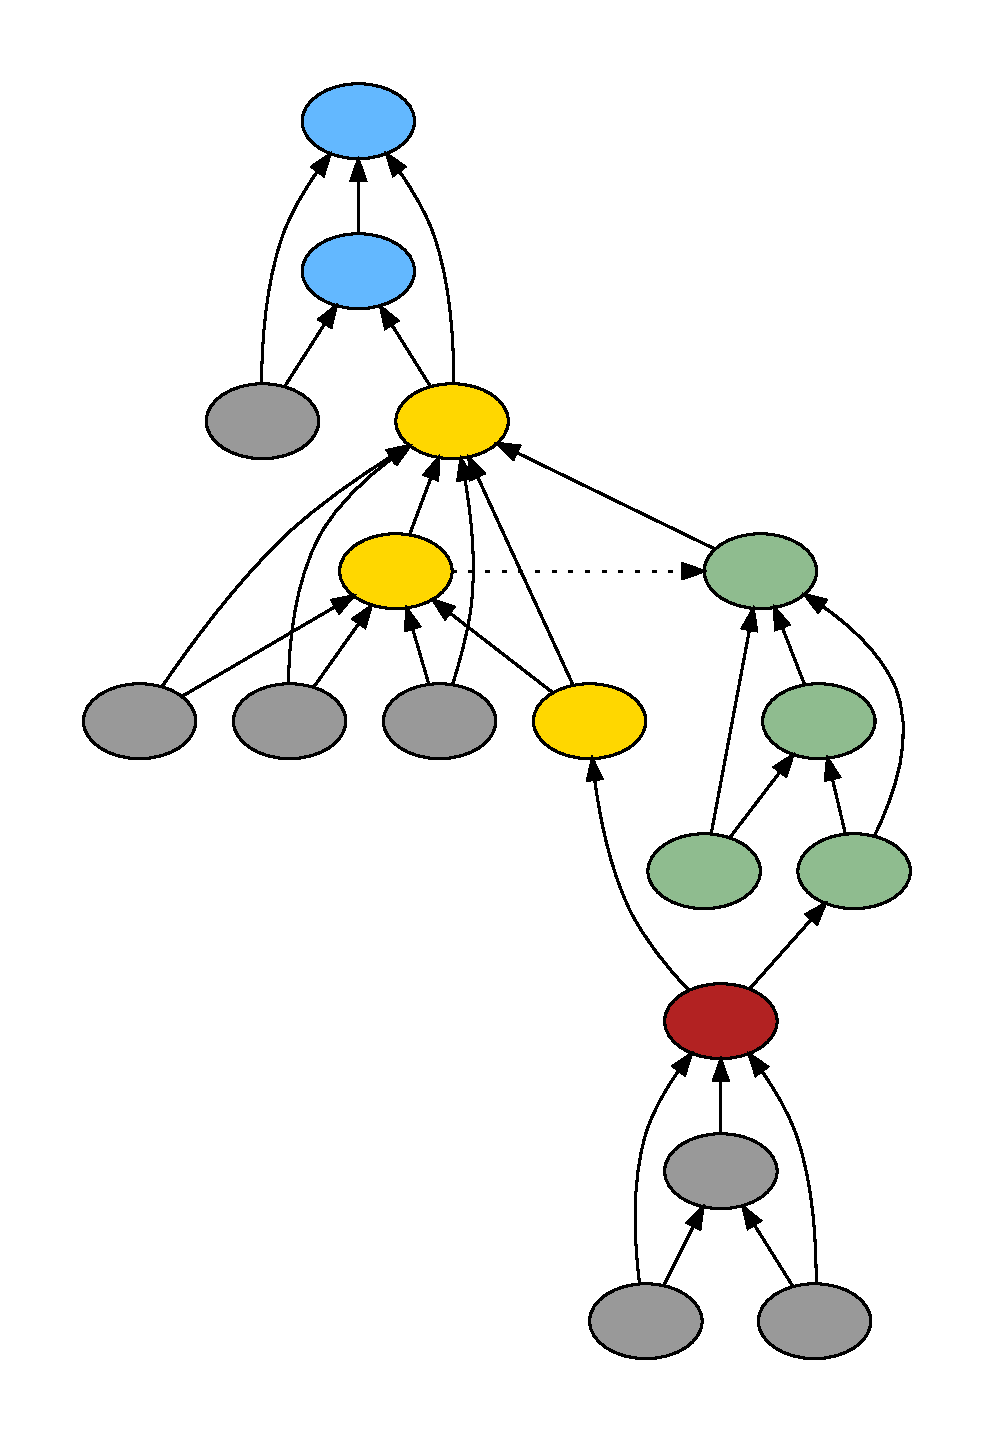
\includegraphics[width=200pt,height=200pt]{erg_to_drg/dot2.pdf}
\label{fig:scaffold_disabled}

}

%

\caption{The two stages of constructing a scaffold}

\label{fig:scaffold}
\end{figure}


%%%%%%%%%%%%%%%%%%%%%%%%%%%%%%%%%%
%%%%%%%%%%%%%%%%%%%%%%%%%%%%%%%%%%
%%%%%%%%%%%%%%%%%%%%%%%%%%%%%%%%%%

\begin{figure}[ht]
\centering

\subfigure
[
A torus with two border nodes. Suppose we regenerate the higher one first, and one of the nodes regenerated makes a simulation request. 
Regen then hands over control to eval in order to evaluate the expression. 
(TODO mark the three nodes that have values, and space-permitting have an
 extra figure to start that just shows the scaffold.)
]
{
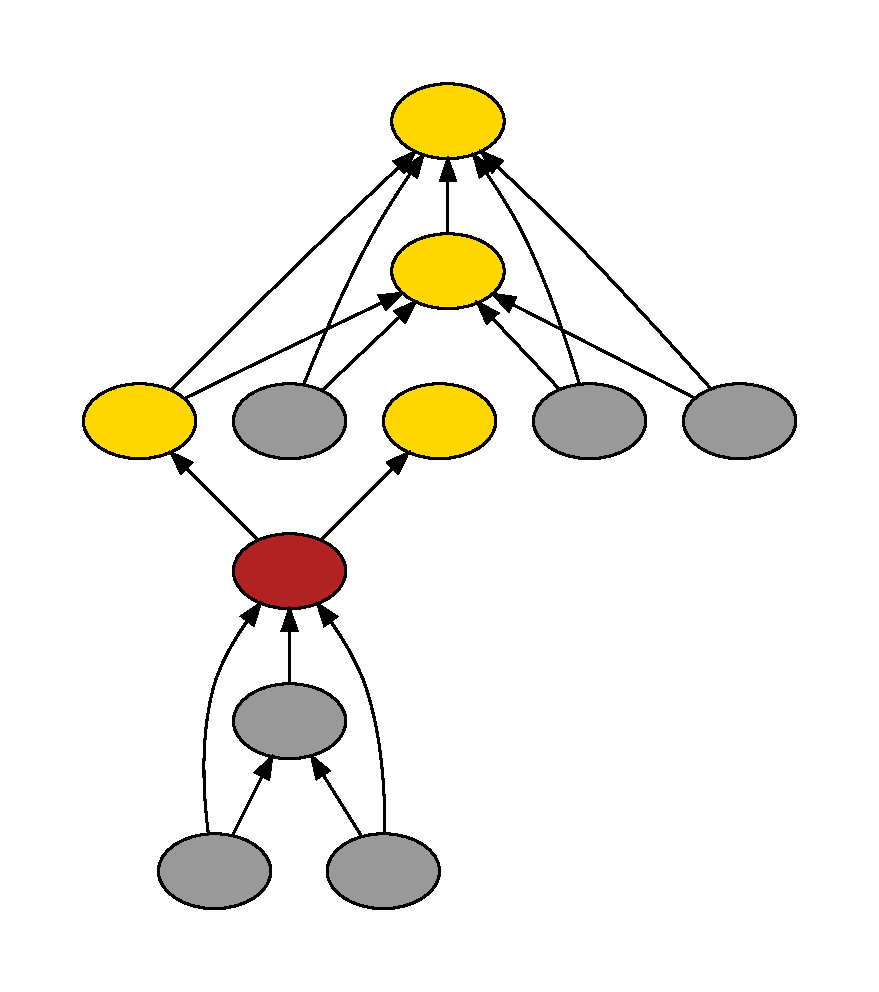
\includegraphics[width=200pt,height=200pt]{regen_to_eval_to_regen/dot6.pdf}

\label{fig:rer_torus}
}

\quad

\subfigure
[
 Evaluating the expression might involve referencing other nodes in the trace, for example to resolve a variable lookup. Those nodes may be in the drg and may not have been regenerated yet, so eval must hand over control to regen to guarantee that all values have been regenerated before they are used.
]
{
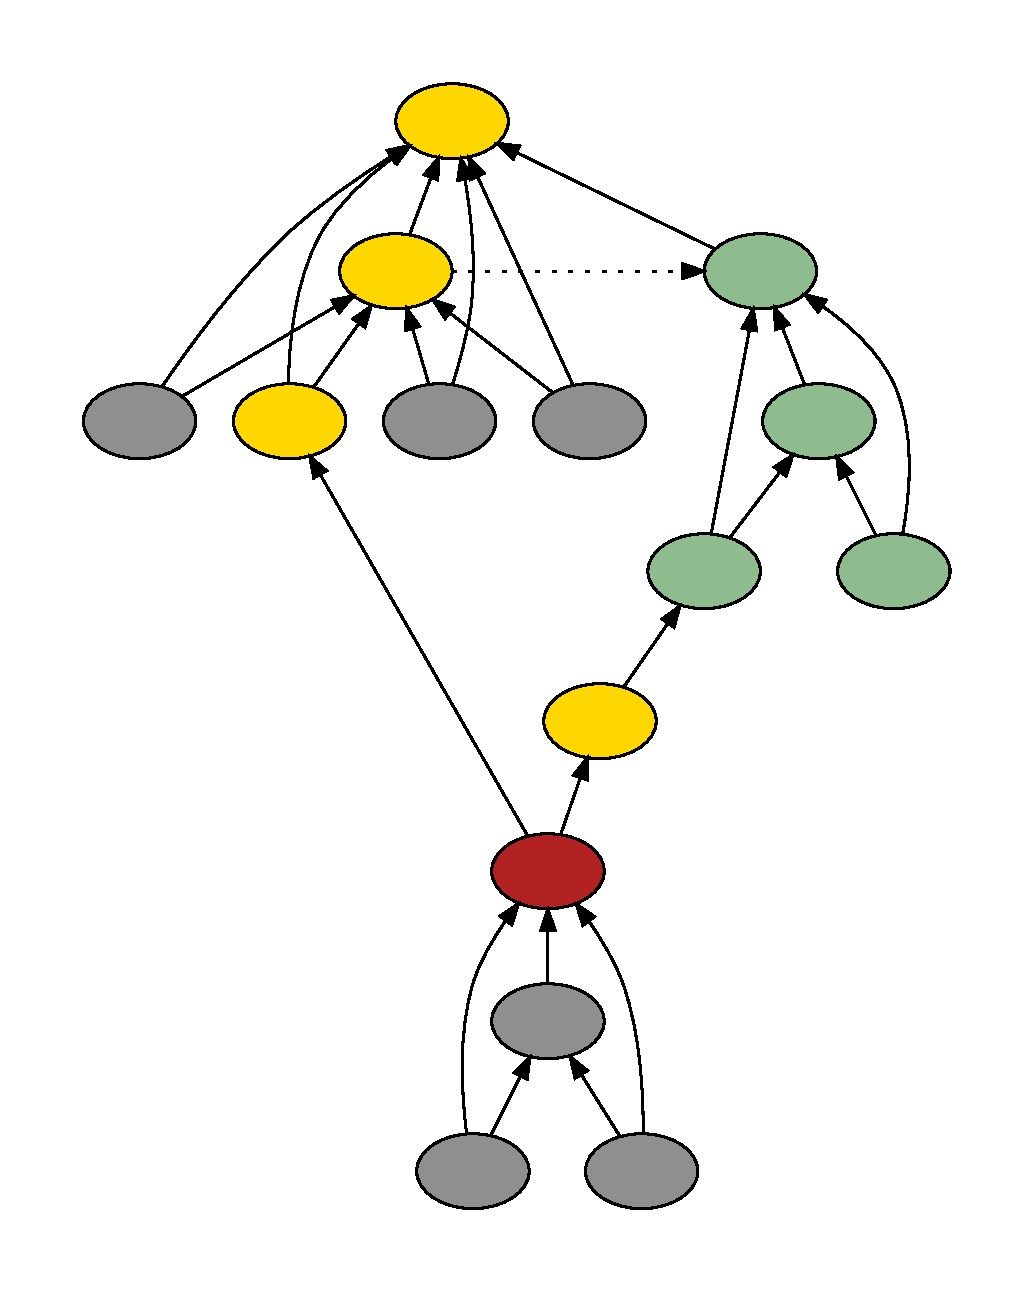
\includegraphics[width=200pt,height=200pt]{regen_to_eval_to_regen/dot2.pdf}
\label{fig:rer_full}

}

%

\caption{Interlacing calls to regen with calls to eval}

\label{fig:rer}
\end{figure}

%%%%%%%%%%%%%%%%%%%%%%%%%%%%%%%%%%
%%%%%%%%%%%%%%%%%%%%%%%%%%%%%%%%%%
%%%%%%%%%%%%%%%%%%%%%%%%%%%%%%%%%%

\begin{figure}[ht]
\centering

\subfigure
[
A large scaffold for sampling a hyperparameter.
]
{
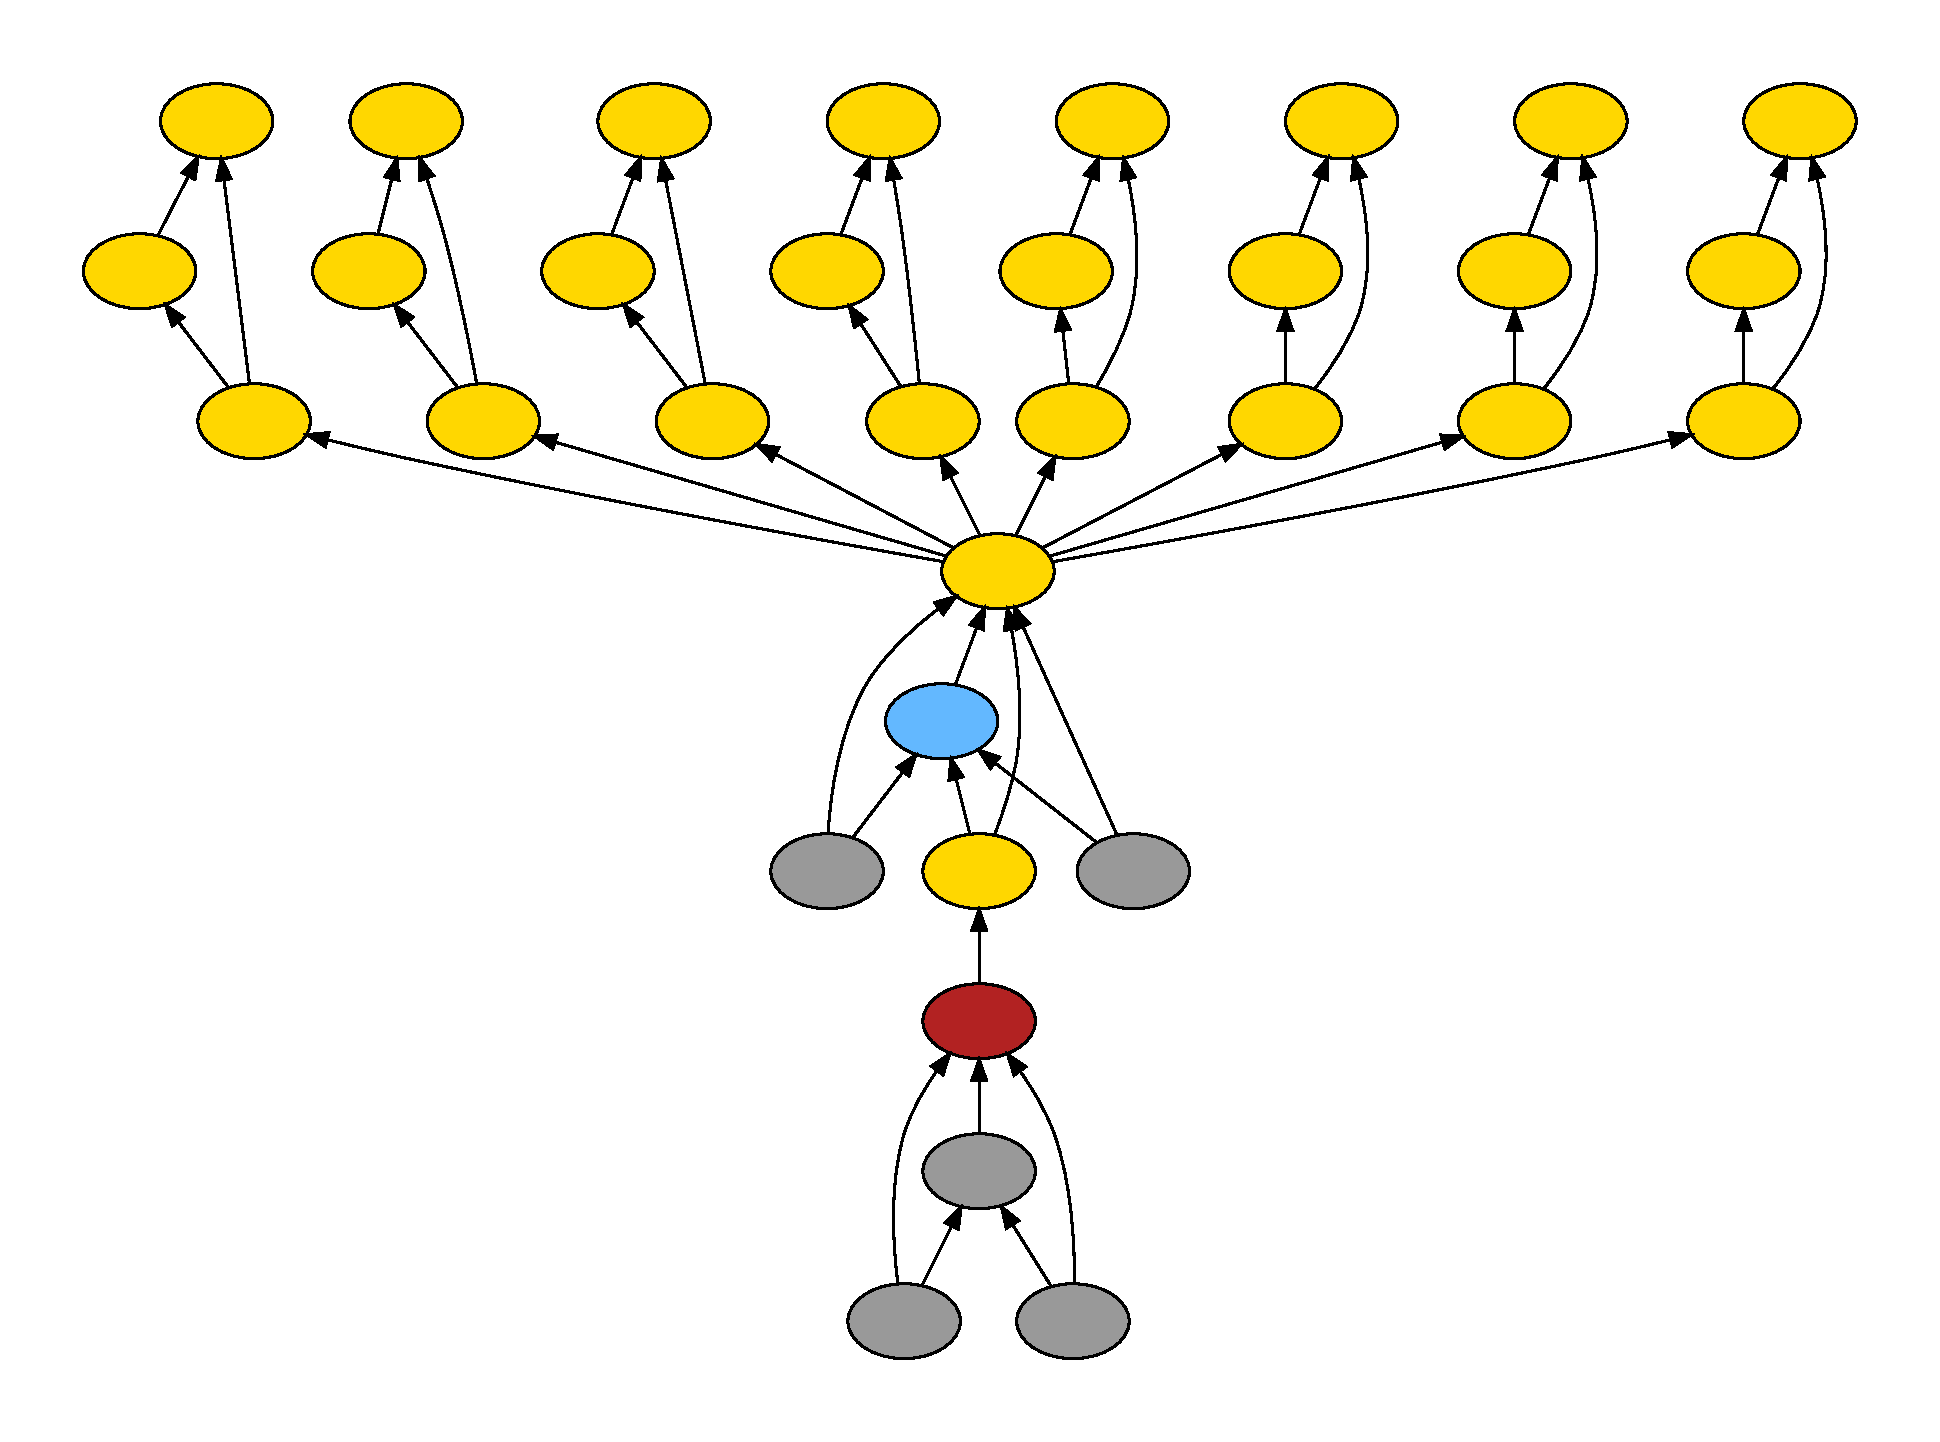
\includegraphics[width=200pt,height=200pt]{aaa_basic_no_aaa/dot2.pdf}
\label{fig:aaa_basic_no_aaa}

}

\quad

\subfigure
[
The application of the maker SP computes the log density of all of its applications for us. We say that the maker SP ``absorbs at applications''.
]
{
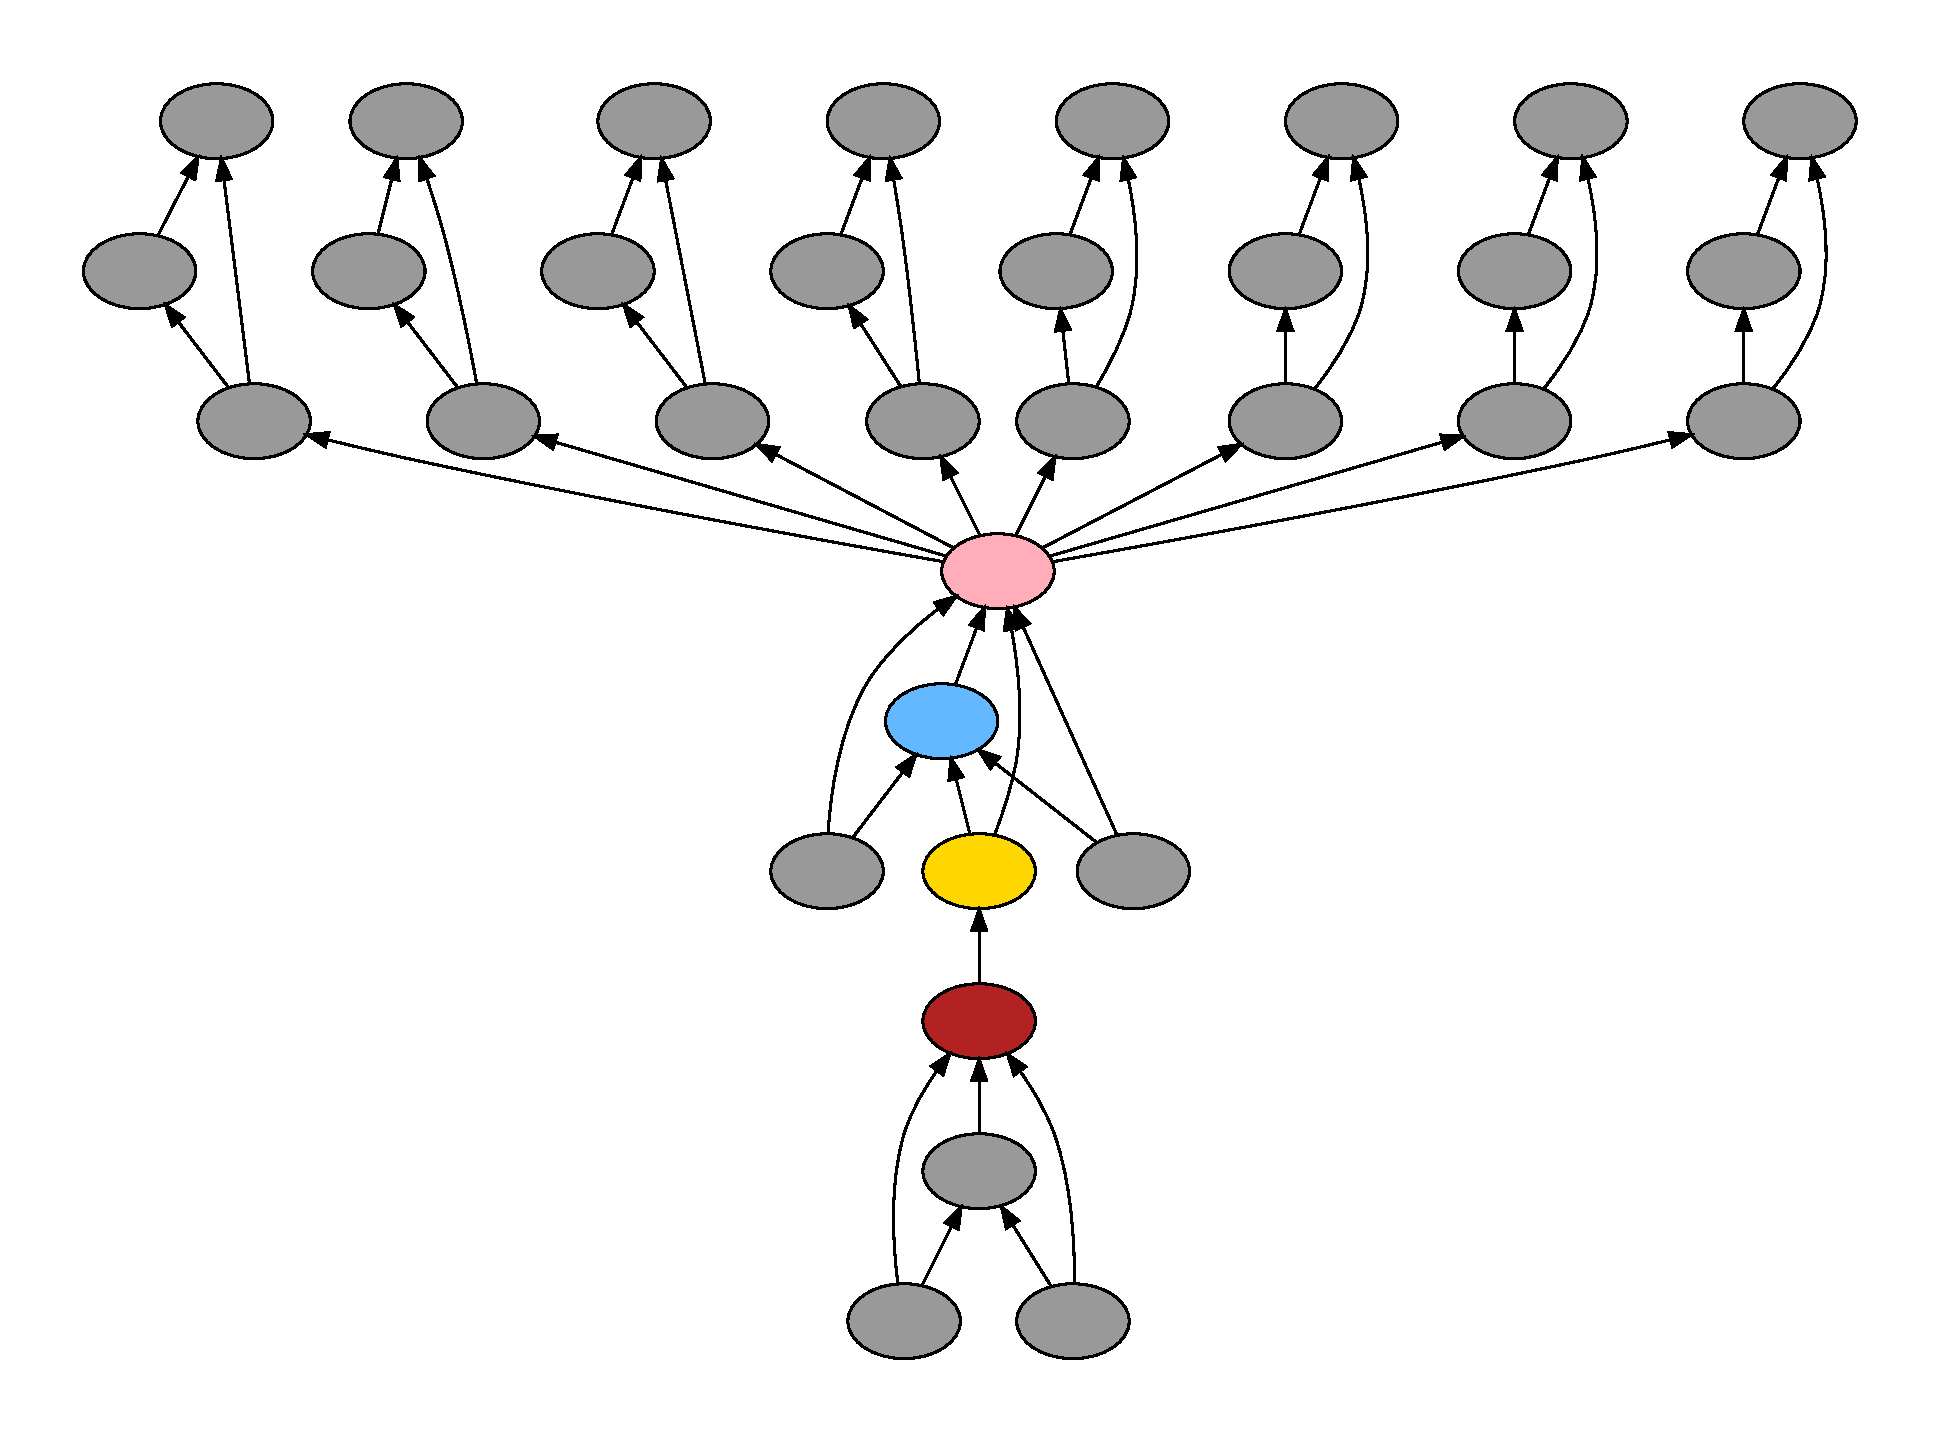
\includegraphics[width=200pt,height=200pt]{aaa_basic_with_aaa/dot2.pdf}
\label{fig:aaa_basic_with_aaa}

}
%

\caption{Absorbing at applications (AAA)}

\label{fig:aaa_basic}
\end{figure}

%%%%%%%%%%%%%%%%%%%%%%%%%%%%%%%%%%
%%%%%%%%%%%%%%%%%%%%%%%%%%%%%%%%%%
%%%%%%%%%%%%%%%%%%%%%%%%%%%%%%%%%%


\begin{figure}[ht]
\centering

\subfigure
[
A scaffold with three border nodes, one of which is absorbing at applications.
]
{
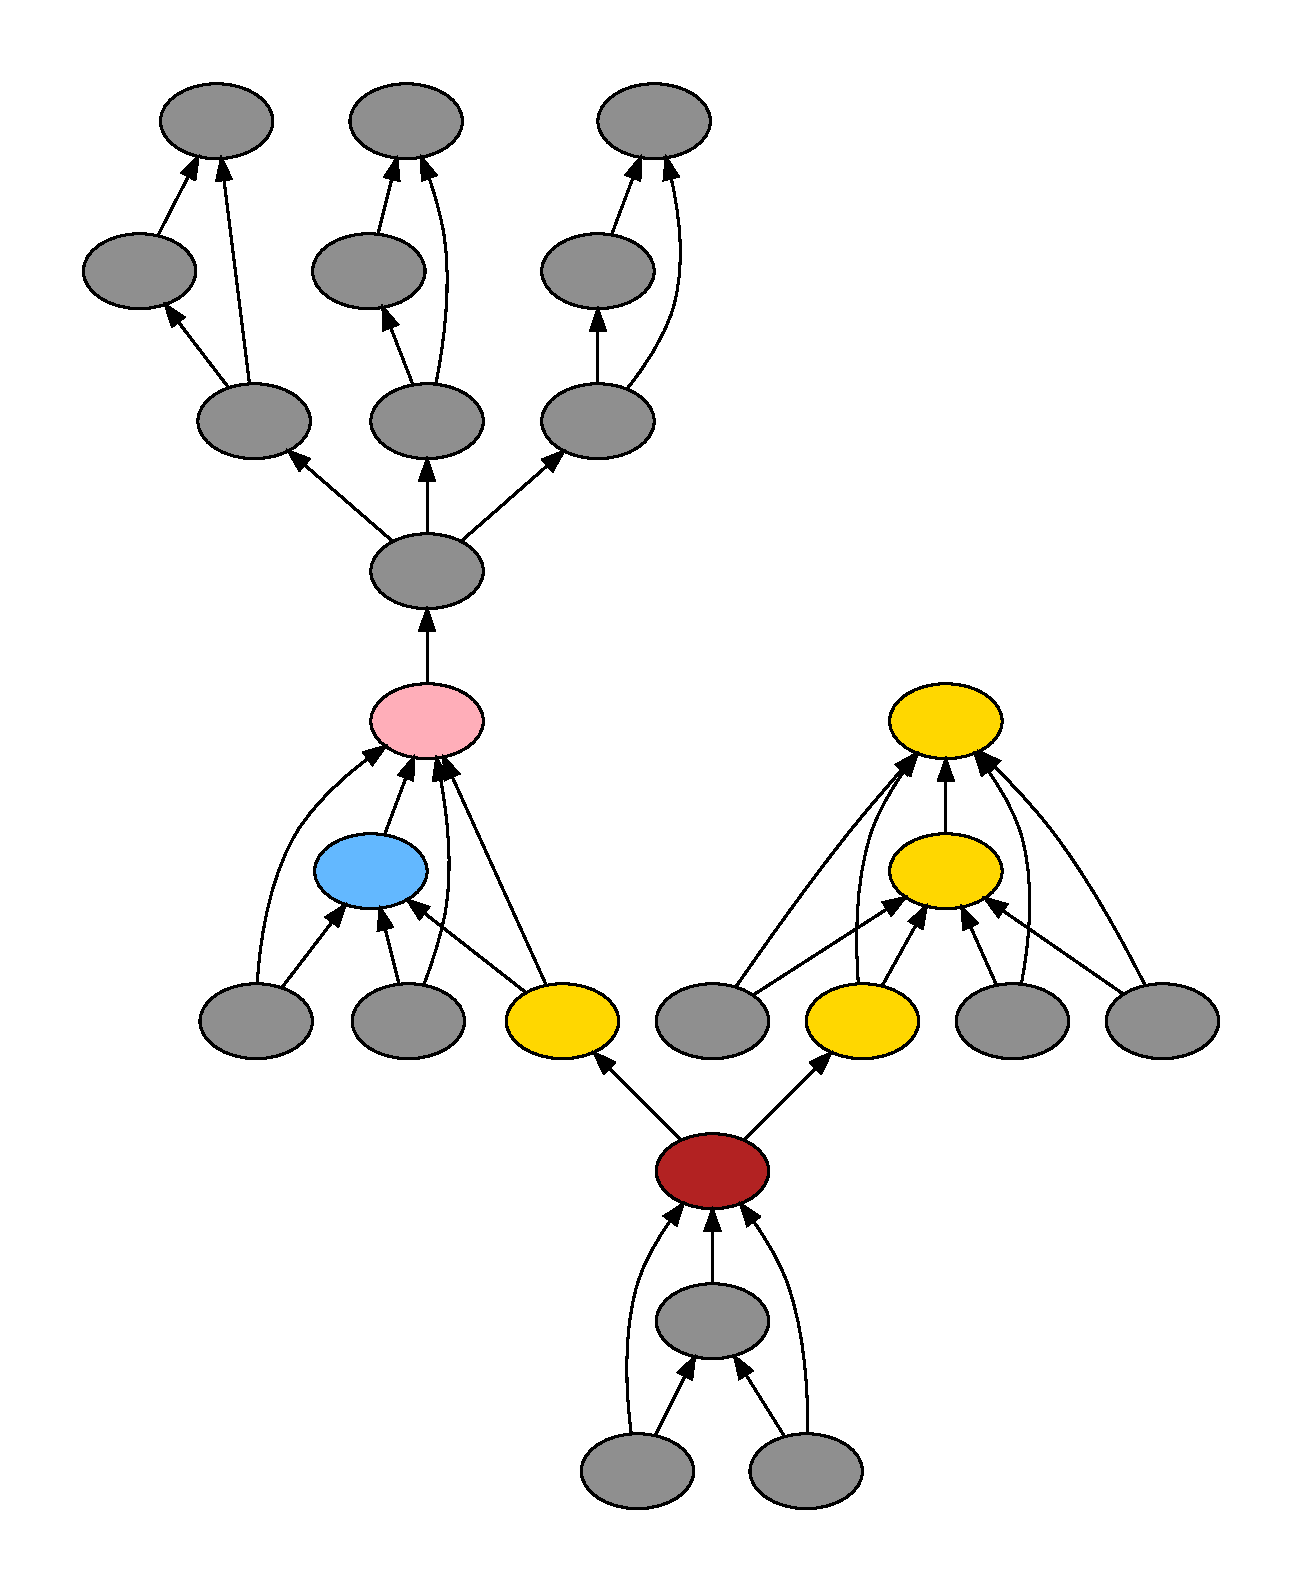
\includegraphics[width=200pt,height=200pt]{aaa_challenge_with_aaa/dot6.pdf}
\label{fig:aaa_challenge_torus}

}

\quad

\subfigure
[
A simulation request may lookup a node that is itself a reference to the aaa node. Even though regen will be called on a node that is not in the drg, the aaa node it refers to must be regenerated nonetheless.
]
{
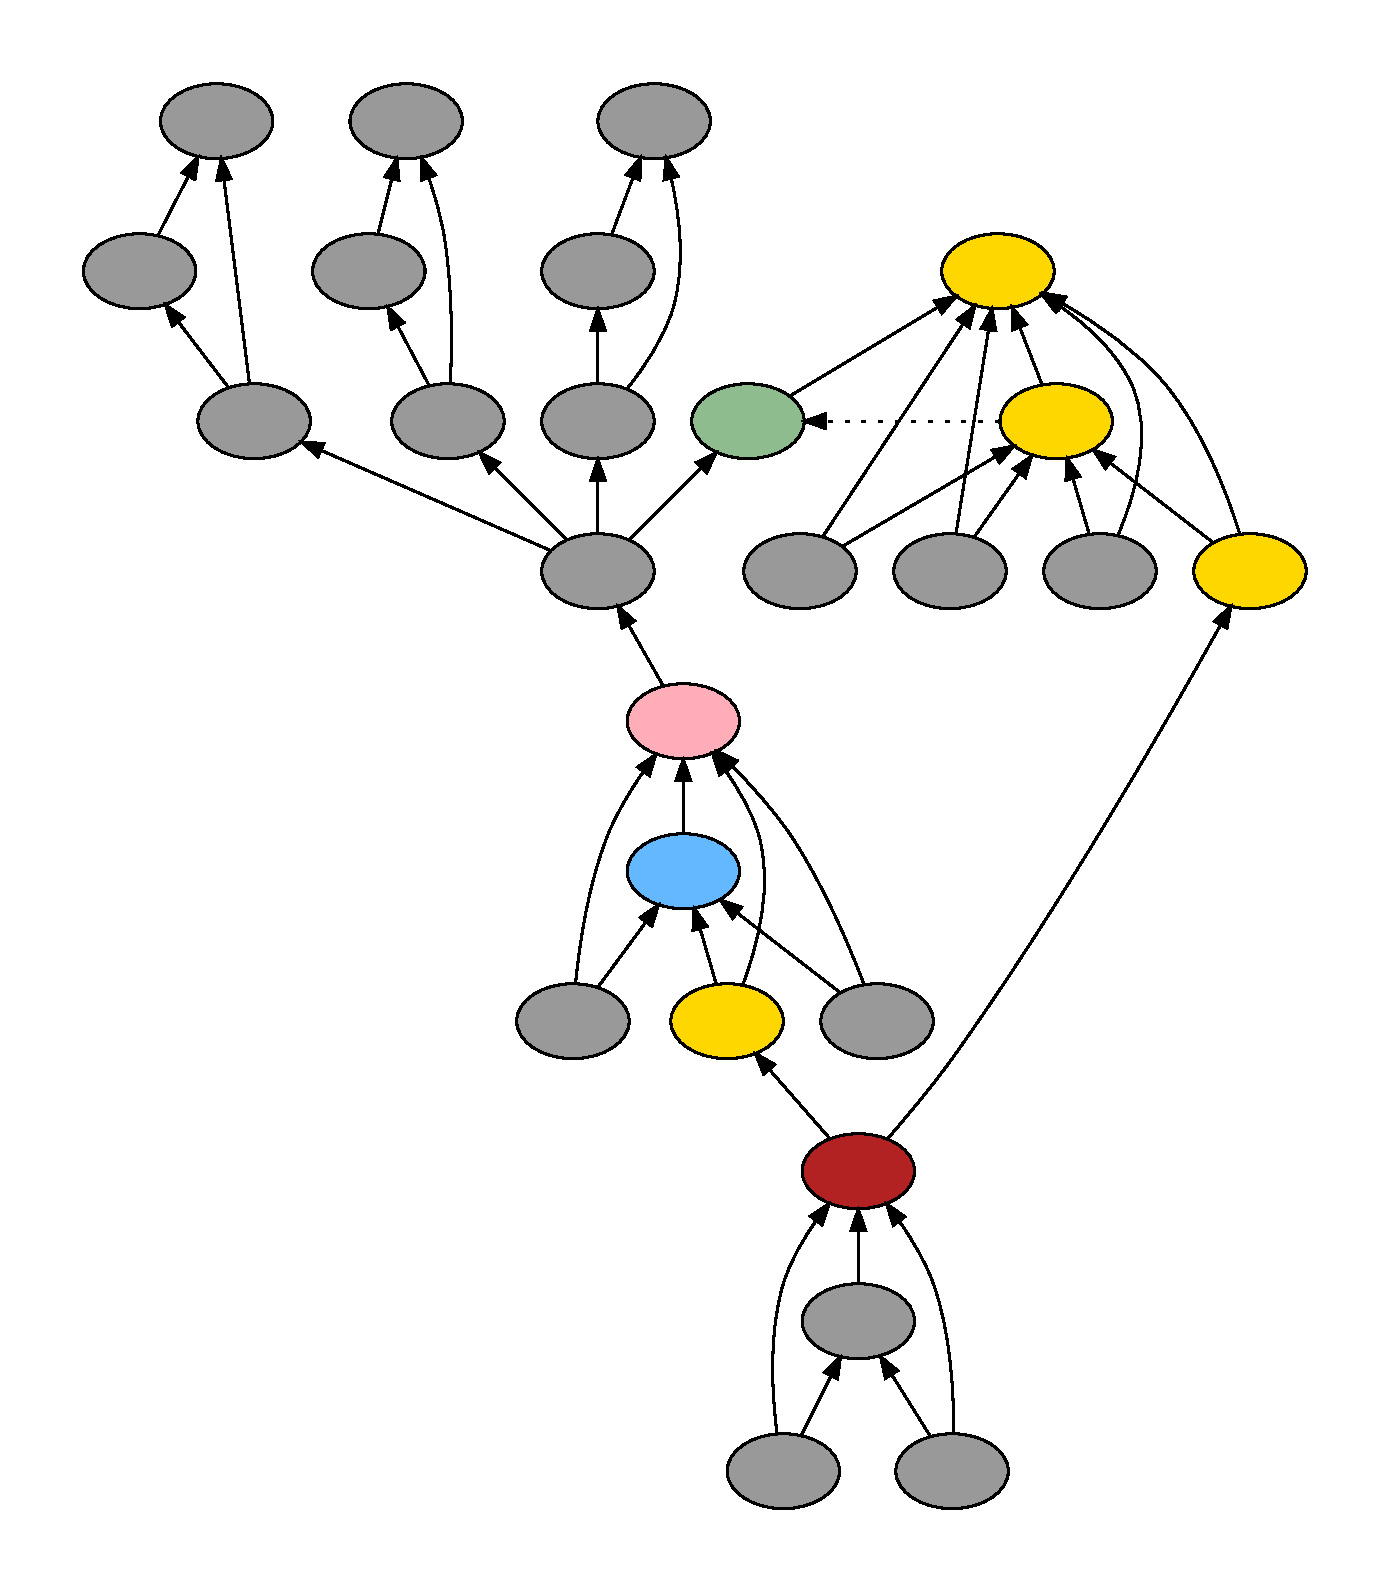
\includegraphics[width=200pt,height=200pt]{aaa_challenge_with_aaa/dot2.pdf}
\label{fig:aaa_challenge_sub}

}
%

\caption{Challenges with absorbing at applications}

\label{fig:aaa_challenge}
\end{figure}


\end{document}
